% this file is called up by thesis.tex
% content in this file will be fed into the main document

%: ----------------------- name of chapter  -------------------------
\chapter{Analiza problemu integracji} % top level followed by section, subsection


%: ----------------------- paths to graphics ------------------------

% change according to folder and file names
\ifpdf
    \graphicspath{{4/figures/PNG/}{4/figures/PDF/}{4/figures/}}
\else
    \graphicspath{{4/figures/EPS/}{4/figures/}}
\fi

%: ----------------------- contents from here ------------------------


Rozdział ten jest podzielony na dwie części. W części pierwszej, zostaną przeanalizowane dostępne syntezatory mowy. Zostaną przedstawione cechy, którymi się charakteryzują oraz ich wady i zalety. W części drugiej zostaną zaprezentowane różne podejścia integracyjne, ich wady i zalety, a także przykładowe architektury dla każdego podejścia. 

\section {Analiza dostępnych silników syntezy mowy}

Tematem tej pracy jest stworzenie platformy, która ułatwi tworzenie i integracje różnego rodzaju aplikacji wykorzystujących syntezę mowy. Tworzenie własnego syntezatora mowy z myślą o tym celu wykracza poza temat, dlatego też platforma zostanie oparta o gotowe syntezatory mowy. Pierwszym krokiem, który został podjęty w celu znalezienia rozwiązań nadających się do użycia, było wyodrębnienie cech opisujących poszczególne syntezatory. Przykładowy zestaw cech, który według autorów dobrze opisuje tego rodzaju systemy znajduje się poniżej: 

\begin{itemize}
	\item \textbf{rodzaj interfejsu}
	\item \textbf{obsługiwana platforma}
	\item \textbf{wydajność}
	\item \textbf{ilość obsługiwanych języków}
	\item \textbf{jakość generowanego dźwięku}
	\item \textbf{cena}
	\begin{itemize}
		\item koszty początkowe(cena zakupu)
		\item koszty użytkowania (opłata za każde użycie)
	\end{itemize}
	\item \textbf{perspektywy rozwoju}
	\item \textbf{łatwość użycia}
\end{itemize}

Ze względu na integrację najważniejszą rolę odgrywa pierwsza z wypisanych cech, a mianowicie rozdaj interfejsu. Ze względu na tą cechę, dostępne syntezatory mowy, można podzielić na następujące grupy: 

\begin{itemize}
	\item lokalne wywołanie
		\begin{itemize}
			\item niestandardowe API
			\item standardowe API - JSAPI, SAPI
		\end{itemize}
	\item komunikacja na poziomie systemu operacyjnego - sockety
	\item protokoły warstwy transportowej modelu TCP/IP - TCP, UDP
	\item specjalistyczne protokoły - MRCP
	\item protokoły ogólnego użytku - HTTP, SOAP, REST
\end{itemize}


Syntezatory należące do pierwszej grupy zazwyczaj działają w obrębie jednej maszyny/urządzenia przez co nie nadają się zbytnio do zastosowania w środowiskach rozproszonych. Co więcej, silniki z podgrupy stosującej niestandardowe API uniemożliwiają szybką ich podmianę jeżeli zajdzie taka potrzeba. 
Grupa druga posiada te same minusy co pierwsza. Dodatkowo, silniki należące do tej grupy, przez zastosowanie niskopoziomowej komunikacji są trudne w użyciu i mogą być mocno uzależnione od konkretnej platformy.
Kolejna grupa w kolejności nadaję się już do zastosowania w środowisku rozproszonym, jednak przez stosowanie protokołów niskopoziomowych zastosowanie rozwiązań z tej grupy jest dość trudne. Dodatkowo, mogą się pojawić problemy z używaniem niestandardowych portów - komunikacja taka może zostać zatrzymana przez firewall. Jednak takie podejście ma też swoje plusy - protokoły te nie zwiększają rozmiaru przesyłanych danych przez dodatkowe nagłówki przez co nie rosną wymagania co do przepustowości sieci.
Rozwiązania należące do następnej w kolejności grupy, przez stosowanie ustandaryzowanych protokołów maja większe szanse na nawiązanie połączenia, nawet w obecności firewalla. Dodatkowym plusem jest fakt, że protokoły te są wyższego poziomu niż protokoły warstwy transportowej, przez co używanie ich jest prostsze. Minusem tych syntezatorów jest mała popularność wykorzystywanych protokołów, przez co znalezienie odpowiednich bibliotek implementujących je, może być trudnym zadaniem.
Ostatnia grupa syntezatorów nadaje się najlepiej ze wszystkich do tworzenia rozproszonej platformy. Posiada ona wszystkie plusy grupy poprzedniej, a dodatkowo protokoły używane przez silniki z tej grupy są na tyle popularne, że znalezienie bibliotek ułatwiających ich obsługę nie stanowi problemu. 

Często się też zdarza, że jeden silnik syntezy mowy posiada wiele interfejsów, przez co jego wartość integracyjna wzrasta. Poniżej znajduje się przykładowa lista dostępnych syntezatorów wraz z interfejsami, które obsługują:

\begin{itemize}
	\item \textbf{Android TTS} - niestandardowe API
	\item \textbf{Festival Speech Synthesis System} - niestandardowe API, JSAPI
	\item \textbf{FreeTTS} - niestandardowe API, JSAPI
	\item \textbf{IVONA SDK} - niestandardowe API, SAPI, TCP, sockety systemu UNIX
	\item \textbf{IVONA Speech Server}  - SAPI, sockety systemu UNIX, TCP
	\item \textbf{IVONA Telecom} - SAPI, MRCP
	\item \textbf{IVONA Speech Cloud} - SOAP, REST
	\item \textbf{Loquendo TTS} - niestandardowe API, SAPI
	\item \textbf{Loquendo embedded TTS} - niestandardowe API, SAPI
	\item \textbf{Loquendo MRCP Server} - MRCP
\end{itemize}


Podjecie decyzji, który syntezator będzie wykorzystany, jak każda inna decyzja dotycząca architektury systemu, nie jest łatwa. Trzeba mieć też na uwadze, że decyzja ta może mieć wpływ na resztę projektu. Autorzy pracy zdecydowali się na stworzenie platformy nie w oparciu o jeden syntezator, czy też o grupę syntezatorów posiadających ten sam interfejs, lecz na stworzenie jej w taki sposób, aby było możliwe zastosowanie w niej różnorodnych silników. 
\section {Architektura}

Znając wymagania które muszą spełniać przedstawione systemy, a także dostępne możliwości jeżeli chodzi o silniki syntezy mowy,  możemy przejść do projektowania architektury tych systemów.

%: ##################### AUTONOMICZNE SYSTEMY #########################################
\subsection {Autonomiczne systemy}
Pierwsze z prezentowanych podejść polega na stworzeniu wyspecjalizowanych, autonomicznych systemów dla każdego problemu z osobna. Architektura ta kompletnie ignoruje problem integracji, dlatego też zwiększa nakład pracy potrzebny do realizacji systemu.  Posiada jednak ona też swoje plusy, które w niektórych przypadkach mogą przemawiać za jej użyciem. 

Systemy multimedialne charakteryzują się specjalnymi wymaganiami w porównaniu do innych tworzonych aplikacji. Najważniejsze z nich to jak najmniejsze opóźnienie. Opóźnienia maja bardzo duży wpływ na to jak użytkownicy odbierają daną aplikacje. Jako przykład niech posłuży platforma telekonferencji. Duże opóźnienia nie tylko utrudniają, lecz również mogą całkowicie uniemożliwić korzystanie z niej. Pierwszy stopień opóźnień wprowadza sieć internet. Czas propagacji sygnału, przepustowość sieci - wszystkie te cechy wpływają na czas potrzebny do przekazania sygnału od nadawcy do odbiorcy. Z powodu wysokiego stopnia złożoności algorytmów, systemy te same z siebie wprowadzają dodatkowy stopień opóźnień. U źródła danych zazwyczaj następuję kompresja danych i kodowanie do odpowiedniego formatu. Po drodze do użytkownika końcowego może nastąpić transkodowanie z jednego formatu na drugi, nawet wielokrotnie. Na końcu, u użytkownika końcowego, następuje proces dekodowania i dekompresji. Każdy z tych procesów czy to u źródła danych, czy u użytkownika końcowego wymaga odpowiedniej ilości czasu. 

Z wyżej wymienionych powodów, ważne jest aby w systemach multimedialnych nie wprowadzać dodatkowych, niepotrzebnych opóźnień, a także, żeby nie zwiększać objętości danych. Podejście autonomicznych systemów pozwala nam na używanie specjalistycznych rozwiązań, które to pomogą nam osiągnąć nasz cel biznesowy, a także spełnienie wymagań stawianych aplikacją multimedialnym. W architekturze tej, część odpowiadająca za logikę biznesową oraz silnik syntezy mowy stanowią jeden autonomiczny system. Bardzo często działają one na jednym urządzeniu, bądź też we wspólnej sieci wewnętrznej. Dzięki takiej architekturze komunikacja miedzy poszczególnymi częściami jest szybka i mniej zawodna. Komunikacja zachodzi bezpośrednio między wymienionymi składnikami systemu, bez żadnych elementów pośrednich. Dodatkowo rozwiązanie takie pozwala w pełni wykorzystać specyfikę danej aplikacji, np. aplikacja na telefon może używać wbudowanych silników syntezy mowy, dzięki czemu nie jest uzależniona od dostępu do internetu - oczywiście  kosztem jakości generowanego dźwięku. 

Wadą takiego rozwiązania jest nakład pracy potrzebny do stworzenia wszystkich systemów. Każdy z nich może być tworzony przy zastosowaniu innych technologii przez co proces projektu i implementacji trzeba powtarzać od podstaw dla każdego z osobna. 
 Kolejną wadą jest fakt że silnik mowy jest częścią systemu. Jeżeli z jakiegoś powodu przestanie on działać, cała aplikacja staje się bezużyteczna. Problematyczna też może się okazać wymiana syntezatora na inny. Z powodu mocnego jego powiązania z resztą, proces ten może wymagać zbyt dużych nakładów pracy.

Ważną kwestią do przemyślenia podczas projektowania jest też rozbudowy systemu. Dotychczas poruszony był tylko temat syntezy mowy, jeżeli  jednak finalny produkt ma być w pełni wartościowy trzeba zastanowić się nad rozszerzeniem go o dodatkową funkcjonalność taką jak:

\label{list:uslugi}
\begin{itemize}
	\item autentykacja
	\item autoryzacja
	\item cachowanie
	\item księgowanie
	\item monitoring
\end{itemize}


Wymienione funkcjonalności mogą być implementowane od zera, dla każdej aplikacji z osobną, lecz wiąże się to z dużym nakładem pracy. Można też skorzystać z gotowych, dostępnych usług dostarczających potrzebnych funkcji. Takie podejście może wiązać się z pewnymi kosztami, ale pozwala na użycie gotowego, sprawdzonego i rozwijanego oprogramowania. Podjęcie decyzji o użyciu zewnętrznych usług, przy zachowaniu autonomiczności każdego z budowanych systemów, wiąże się z integracją każdej usługi ze wszystkimi systemami, które jej wymagają z osobna. Przy założeniu, że tworzone jest \begin{math}n\end{math} aplikacji, i każda z nich będzie korzystała z \begin{math}m\end{math} usług to liczba połączeń aplikacja-usługa, które trzeba stworzyć wynosi  \begin{math}n*m\end{math}, a złożoność tak powstałej sieci wynosi \begin{math}O(nm)\end{math}. Przy założeniu, ze liczba aplikacji jest równa liczbie usług czyli \begin{math}m = n\end{math}, złożoność ta wynosi \begin{math}O(n^2)\end{math}.

 Przykładową architekturę w tym podejściu dla tworzonych systemów przedstawia rysunek \ref{fig:autonomiczne_systemy}

\setlength\fboxsep{20pt}
\setlength\fboxrule{1pt}
\begin{figure}[!h]
	\centering
	\fbox{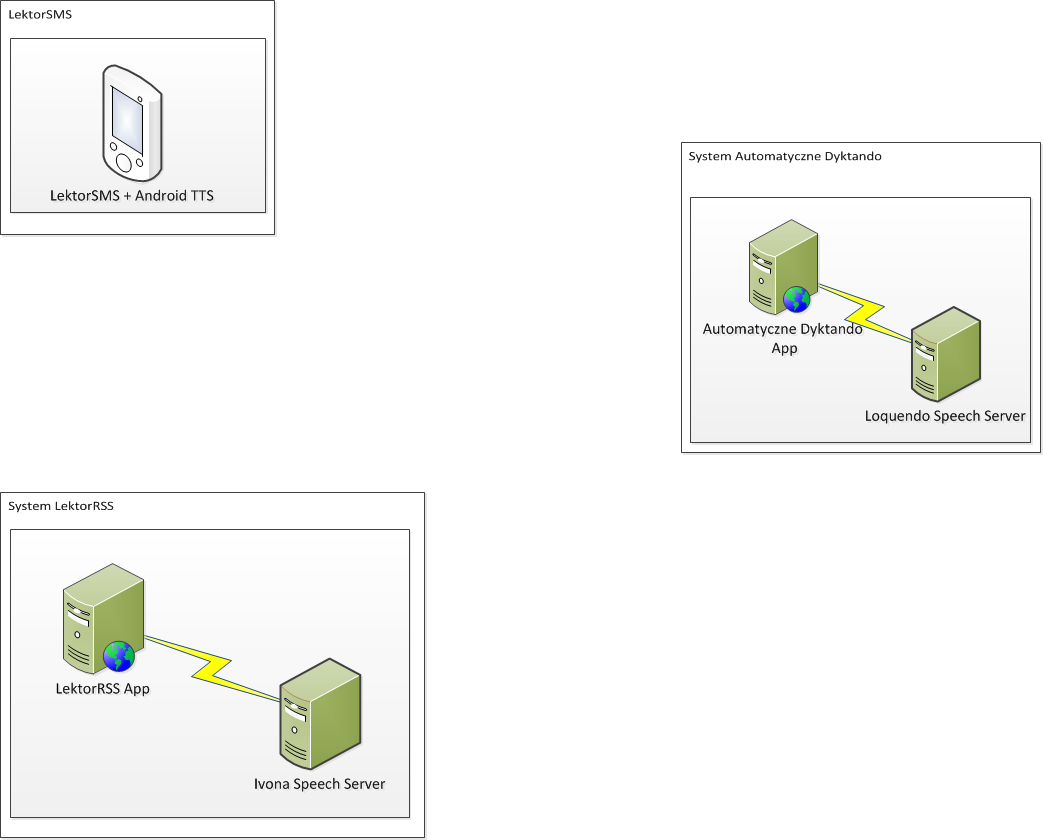
\includegraphics[scale=0.45]{wyspecjalizowane_rozwiazania.png} }
	\caption{Architektura - Autonomiczne systemy}\label{fig:autonomiczne_systemy}
\end{figure}

Podejście autonomicznych aplikacji jest  skupione na konkretnych systemach, a nie na integracji ich w istniejącym środowisku. Można nawet stwierdzić, że w tej architekturze w ogóle nie występuje element integracji. Jednakże, rozwiązanie to ma też swoje plusy. Przy tym podejściu, powstające systemy są lepiej dostosowane do stawianych przed nimi zadań, ale także wymagają większych nakładów pracy i są ciężkie w rozbudowie. Kolejna prezentowana architektura,  patrzy na problem z nieco innej perspektywy. Nie jest one aż tak  skupiona na tworzonych systemach, lecz na ich współistnieniu i współpracy z innymi usługami w środowisku SOA.

%: ##################### HUB and Spoke #########################################
\subsection {Podejście zorientowane na usługi}
Dzięki postępowi technologicznemu przepustowość łączy internetowych wciąż wzrasta. Dzięki temu, to co parę lat temu było nie osiągalne dziś jest normą. Powstają nowe rodzaje usług, które kiedyś nie mogłyby zostać zrealizowane, przy tworzeniu zaś niektórych aplikacji, to co kiedyś było problemem i na czym skupiali swój wysiłek twórcy oprogramowania, dzisiaj schodzi na drugi plan. Z drugiej jednak strony zwiększają się wymagania użytkowników co do jakości multimediów, co wymuszą wprowadzanie coraz to nowszych formatów, które mają większe wymagania co do przepustowości łączy internetowych. Czasami jednak systemy multimedialne nie mają takich ścisłych wymagań co do wielkości opóźnienia. W ich przypadku opóźnienie nawet rzędu kilkudziesięciu sekund nie stanowi problemu i jest akceptowalne przez użytkowników. W takim wypadku nie trzeba skupiać się na szukaniu idealnego rozwiązania dla danego problemu, lecz można skupić się na stworzeniu architektury która ułatwi i przyspieszy budowanie systemów realizujących różne cele biznesowe.

Przy takim podejściu zazwyczaj pojawia się problem integracji budowanej aplikacji z istniejącymi już usługami. Często też, budowany system jest całkowicie problemem integracyjnym, czyli wszystkie składowe usługi potrzebne do realizacji celu biznesowego są dostępne, a jedyne zadanie stawiane budowanemu systemowi to odpowiednia ich integracja. Taka architektura ułatwia parę kwestii, ale w zamian wprowadza także nowe, specyficzne dla siebie problemy. Głównym problemem jest różnorodność dostępnych podsystemów. Każdy z nich może być stworzony przy użyciu innych technologii (Java, COM, .Net, CORBA, ICE, itp.), działać na innej platformie (MS WINDOWS, LINUX, SOLARIS) i co najważniejsze może wykorzystywać inne protokoły do komunikacji (RPC, SOAP, własnościowe protokoły, itp). Z tego powodu decyzja o zastosowaniu tej architektury nie może zostać podjęta zbyt pochopnie i powinna oparta na pewnych kryteriach. Przykładowe kryteria to:  \cite{hohpewoolf2003} 

\begin{itemize}
	\item \textbf{powiązanie aplikacji} - integracja aplikacji powinna minimalizować powiązania i zależności między nimi, co pozwoli na swobodne rozwijanie każdej aplikacji z osobna. Ściśle powiązane aplikacje współdziałają przy wielu założeniach z każdej ze stron. Jeżeli któraś z aplikacji zostanie zmieniona i założenia co do niej przestaną być spełnione wtedy cała integracja przestanie działać. Dlatego też, projektowane interfejsy powinny być na tyle specyficzne aby umożliwiały implementację użytecznych funkcjonalności, lecz także na tyle ogólne aby umożliwiały zmianę implementacji, jeżeli zajdzie taka potrzeba.
	\item \textbf{poziom ingerencji} - podczas integracji aplikacji, powinno się minimalizować zarówno zmiany w samej aplikacji jak i ilość kodu tworzonego na rzecz integracji. Jednak bardzo często zarówno zmiany w aplikacji jak i tworzenie dodatkowego kodu odpowiadającego za integracje jest nieuniknione aby uzyskać odpowiednią funkcjonalność. Rozwiązania mniej ingerujące w aplikacje mogą nie zapewniać integracji w odpowiednim stopniu.
	\item \textbf{wybór technologii} - do wyboru mamy mnóstwo technologii integracyjnych, które różnią się od siebie wymaganiami co do specjalistycznego sprzętu i do oprogramowania. Nie które z nich są wymienne między sobą, natomiast wybranie innych może prowadzić na zamknięcie się na dane rozwiązanie. Jeżeli podejmie się decyzje o zastosowaniu którejś z gotowych technologii integracji może ona znacząco zwiększyć koszt całego system. Z drugiej strony, integracja od podstaw zazwyczaj kończy się większym nakładem pracy niż początkowo planowano i może oznaczać odkrywanie koła na nowo.
	\item \textbf{format danych} - integrowane aplikacje muszą posługiwać się tym samym formatem podczas wymiany danych. Dostosowywanie istniejących aplikacji do jednolitego formatu danych może być bardzo trudne, albo wręcz nie możliwe. Inną opcją jest wprowadzenie elementu pośredniego, którego celem będzie tłumaczenie danych z jednego formatu na drugi. Problemem powiązanym z opisanym w tym podpunkcie jest problem rozszerzalności i rozwoju formatu danych - jak format danych może się zmieniać z biegiem czasu i jak te zmiany wpłyną na integrowane aplikacje.
	\item \textbf{żywotność danych} - zastosowane rozwiązanie integracyjne powinno minimalizować czas pomiędzy udostępnieniem danych przez jedną aplikację, a pobraniem tych danych przez drugą. Można to osiągnąć poprzez częstą wymianę małych porcji danych, jednakże takie podejście może zmniejszyć wydajność całego systemu. Opóźnienia związane z wymianą danych muszą zostać wzięte pod uwagę podczas planowania integracji. W idealnym systemie, aplikacja odbiorca zostanie poinformowana jak tylko dane będą dostępne. Im dłuższy czas miedzy publikacją a konsumpcją danych tym większa szansa, że aplikacje ulegną rozsynchronizowaniu.
	\item \textbf{rodzaj komunikacji} - przetwarzanie komputerowe jest w dużej większości synchroniczne - to znaczy, że jedna procedura wywołuje drugą ( pod-procedurę) i czeka na jej wykonanie. W systemach rozproszonych, wywołania mają charakter zdalny, co powoduje, że są o wiele wolniejsze od wywołań lokalnych. Z tego powodu, oczekiwanie na zakończenie wywołania, jest często niepożądane. W takim wypadku można wykorzystać podejście asynchroniczne - procedura wywołuje pod-procedurę, lecz nie czeka na jej zakończenie, jak to było w wypadku wywołania synchronicznego, tylko wraca do swojego przetwarzania. Kiedy pod-procedura zakończy przetwarzanie, informuje o tym procedurę wywołująca i zwraca jej wynik. Komunikacja asynchroniczna może zwiększyć wydajność całego systemu, ale również może uczynić go bardziej złożonym.
	\item \textbf{poziom niezawodności} - komunikacja zdalna jest nie tylko wolniejsza, ale również bardziej zawodna niż lokalne wywołania funkcji. Kiedy procedura wywołuje pod-procedurę w obrębie jednej aplikacji, jest pewne, że jest ona dostępna. Takie założenie nie musi być spełnione jeżeli chodzi o zdalne wywołania - zdalna aplikacja może nie działać w chwili wywołania, albo połączenie z siecią może być chwilowo niedostępne.
\end{itemize}

Do wyboru dostępnych jest dużo różnych technologii integracyjnych. Niektóre z nich są niezależne od platformy, inne zaś wymagają specyficznego systemu operacyjnego. Niektóre z nich są darmowe i otwarte, inne zaś płatne i oparte na własnościowych patentach i protokołach. Każda z nich ma swoje plusy i minusy dlatego trzeba wybrać tą która najlepiej nadaje się dla określonego celu. Dodatkową opcją jest tworzenie swojego systemu integracji od zera. Jednak ze względu na to iż takie rozwiązanie jest czasochłonne, a także celowość takiego podejścia stoi pod znakiem zapytania, to nie jest ono brane pod uwagę podczas projektowania systemu. 
Dostępne rozwiązania można podzielić na cztery grupy: \cite{chappell2004}

\begin{itemize}
	\item serwery aplikacji
	\item brokerzy EAI
	\item własne rozwiązania oparte na  MOM
	\item ESB
\end{itemize}

Pierwsze dwie grupy rozwiązań oparte są na modelu piasty i szprych (\textit{"Hub and Spoke"}). W modelu tym poszczególne części systemu ułożone są na wzór koła rowerowego, w którym przebieg danych odbywa się wzdłuż szprych połączonych z położoną w centrum piastą. Zaletą takiego rozwiązania jest scentralizowanie takich funkcji systemu jak zarządzanie czy routowanie wiadomości,  które to są zaimplementowane w węźle centralnym(piaście). Dzięki temu poszczególne węzły - szprychy wyposażone są tylko w niezbędną dla nich funkcjonalność. Kolejną zaletą jest ilość połączeń którą trzeba zrealizować w takim modelu. Przy założeniu, że tworzone jest \begin{math}n\end{math} aplikacji i każda z nich musi komunikować się z resztą to suma połączeń które trzeba zrealizować wynosi \begin{math}n\end{math},a złożoność powstałej sieci wynosi \begin{math}O(n)\end{math}. Jest to znacznie lepszy wyniki niż przy sieci typu punk-punkt, w której to ilość połączeń do zrealizowania wynosi \begin{math}\frac{n (n- 1)}{2}\end{math}, a złożoność jej wynosi wynosi  \begin{math}O(n^2)\end{math}. Wadami takiego rozwiązania jest słaba skalowalność, istnienie pojedynczego punktu awarii w postaci węzła-piasty oraz wprowadzenie dodatkowego opóźnienia - jeden dodatkowy przeskok w porównani z bezpośrednią komunikacją między aplikacjami.

\setlength\fboxsep{20pt}
\setlength\fboxrule{1pt}
\begin{figure}[!h]
	\centering
	\fbox{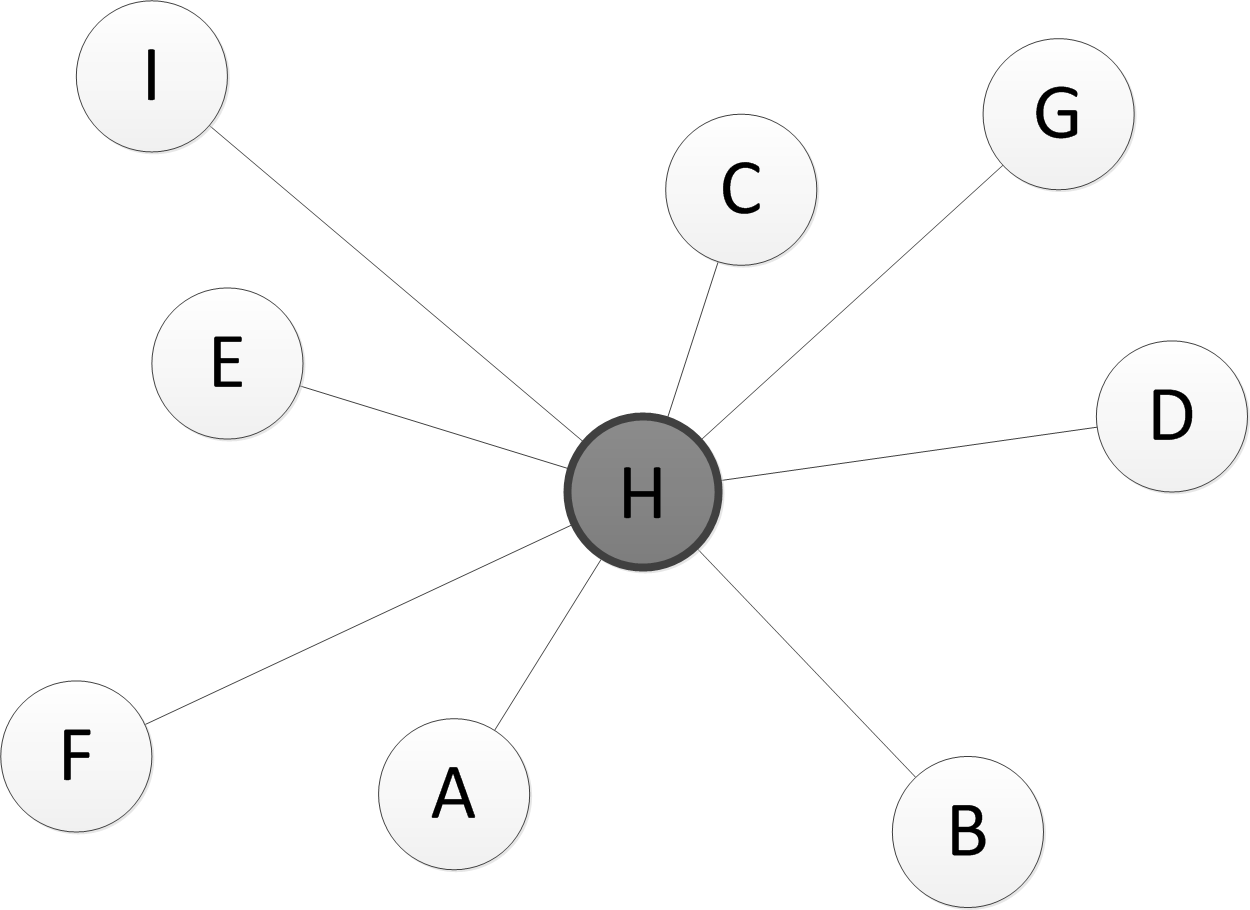
\includegraphics[scale=0.35]{hub_and_spoke_model.png} }
	\caption{Model "piasta i szprychy"}\label{fig:hub_and_spoke}
\end{figure}

Rozwiązania oparte na serwerach aplikacji upraszczają implementację komunikacji ponieważ serwery te zazwyczaj są wyposażone w obsługę standardowych protokołów takich jak HTTP czy SOAP. Minusem tych rozwiązań jest to, że logika integracyjna i logika biznesowa przeplatają się nawzajem, a także poszczególne części systemu są dość mocno ze sobą powiązane co zmniejsza elastyczność systemu.

Zastosowanie brokerów EAI posiada wszystkie wady i zalety co użycie serwerów aplikacji, lecz dzięki rozdzieleniu logiki integracyjnej od biznesowej poszczególne części systemu są ze sobą mniej powiązane. Ma to pozytywny wpływ na jakość systemu, a także ułatwią jego dalszą rozbudowę i rozwój.

Rozwiązania oparte na MOM pozwalają na luźne łączenie poszczególnych systemów a także na asynchroniczną komunikację między nimi. Rozwiązania te zazwyczaj nie posiadają wysoko poziomowej warstwy abstrakcji nad logiką routowania co fragmentami wymusza programowanie na dość niskim poziomie. Z tego też powodu, w rozwiązaniach tych, podobnie jak w rozwiązaniach opartych na serwerach aplikacji logika integracyjna jest przeplatana z biznesową, co utrudnia utrzymywanie i rozwijanie takiego systemu.

Ostatnia grupa rozwiązań jest oparta na ESB. Jest to najnowsza z wyżej opisanych technologii. Dzięki doświadczeniu zdobytemu przy projektowaniu i użytkowaniu wyżej opisanych technologii, udało się stworzyć rozwiązanie, które nie posiada tych samych wad co jej poprzedniczki. Technologia ESB dostarcza mocno rozproszone środowisko, które pozwala na tworzenie dobrze skalowalnych systemów. Kolejnym plusem tej technologii jest oddzielenie logiki biznesowej od integracyjnej takiej jak routing czy transformacja danych, dzięki czemu tworzone systemy są łatwiejsze w utrzymaniu i rozbudowie, a także nie są ściśle związane z jedną technologią. 

\setlength\fboxsep{20pt}
\setlength\fboxrule{1pt}
\begin{figure}[!h]
	\centering
	\fbox{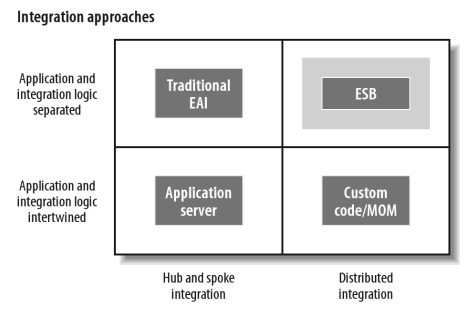
\includegraphics{podejscia_integracyjne.png} }
	\caption{Różne podejścia integracyjne  \cite{chappell2004}}\label{fig:podejscia_integracyjne}
\end{figure}


\newpage
\section*{Podsumowanie}
W powyższym rozdziale zostało przedstawione wiele podejście do problemu integracji aplikacji. Z powodu dużej ich różnorodności, ciężko stwierdzić, że któreś z nich jest zdecydowanie lepsze od reszty. Decyzja o wyborze konkretnej technologii powinna być dopasowana do rozwiązywanego problemu. Dzięki opisanym wadom i zaletom każdej z architektur można lepiej wybrać tą która najlepiej będzie odpowiadać stawianym wymaganiom. Spośród czterech wyżej opisanych podejść, autorzy wybrali podejście ESB jako najlepiej spełniające wymagania stawiane tworzonemu systemowi. Jeżeli chodzi o silniki mowy, autorzy pracy nie chcą skupiać się na jednym  konkretnym, lecz stworzyć system, który pozwoli w łatwy sposób na integracje dowolnego silnika syntezy mowy. Powyższy rozdział daje solidne podstawy do rozpoczęcia projektowania i implementacji systemu  zgodnie z wybranym podejściem.

%ksiazka ESB strony 4,5 

%opiszemy to podejscie i potem opiszemy, ze jest bardzo fajne, opiszemy rodzaje, jak ewoluowało, i na koncu opiszemy esb, a potem konkrety dla naszej aplikacji. Obrazki w ksiazce ESB
%ESB strona 34 - czemu własnościowe rozwiązania sa do dupy 



%\subsection {Szyna} 

%Przedstawienie jak to wyglada( kropki serwisy , komunikują sie z roznymi innymi serwisami, dodatokwe serisy: accounting itd)

%Wymagania stawiane rozwiazaniom integracyjnym , Czy warto integrować ? (book1.pdf chapter 2)

%Integracja systemow multimedialnych ??

%Rozwiazania ?

%Brak integracji

%integracja EAI - hub and spikes (scentralizowany punk, single point of failure. słabo scalowalne)

%SOA - ESB 




%service activator (request od clienta)


% ---------------------------------------------------------------------------
%: ----------------------- end of thesis sub-document ------------------------
% ---------------------------------------------------------------------------

